\documentclass[senior,etd,astronomy]{BYUPhys}


% ------- Fill in these fields for the preliminary pages --------
% For Senior and honors this is the year and month that you submit the thesis
% For Masters and PhD, this is your graduation date
  \Year{2006}
  \Month{June}
  \Author{Justin Peatross and Michael Ware}

% If you have a long title, split it between two lines using the \\ command.
% A multiple line title should be an "inverted pyramid" with the top line(s)
% longer than the bottom.
  \Title{Incredibly Useful Advice for Physics Students\\ Writing a Senior Thesis}

  \Advisor{Albert Einstein}

  \Abstract{The abstract is a \emph{summary} of the thesis,
  \emph{not an introduction}. Keep in mind that abstracts are
  often published separately from the paper they summarize. In
  your abstract, give a concise synopsis of the work,
  emphasizing the conclusions; you need not include the
  supporting arguments for the conclusions. The purpose of the
  abstract is to help prospective readers decide whether to
  read your thesis, but your goal is not necessarily to
  persuade people to read your thesis. A successful
  abstract enables people to get an accurate overall view of
  your work without needing to read it.

  Usually, an abstract contains only one paragraph, but it can
  have more if absolutely necessary. Remember to state the
  subject of the paper immediately followed by a summary of the
  experimental or theoretical results and the methods used to
  obtain them. Avoid equations, graphics, and citations; if a
  citation is essential it must be cited fully within the
  abstract. Keep the abstract factual. Avoid vague statements
  like, ``Conclusions are drawn," or ``the significance of the
  experiment is discussed."  State the conclusions and findings
  outright in the abstract.}

 \Keywords{senior thesis, undergraduate research, templates}

% To opt not to have an acknowledgment page,
% give the option "noacknowlegments" to BYUPhys

  \Acknowledgments{
    This page is optional. You may acknowledge whom you will---your
    advisor, colleagues, family members. Please keep acknowledgments
    in good taste. I would like to acknowledge Dr. Kristine Hansen and Dr.
    Elizabeth Hedengren, whose Advanced Writing Seminar motivated this project.
    I also wish to thank Jean-Fran\c{c}ois Van Huele, Steven Turley, and Ross
    Spencer for reviewing this document and for ripping it to shreds
    as every good advisor should do to a thesis draft.
  }

\begin{document}

 % Start page counting in roman numerals
 \frontmatter

 % This command makes the formal preliminary pages.
 % You can comment it out during the drafting process if you want to save paper.
 \makepreliminarypages

 % Make the table of contents.
 \tableofcontents

 % Start regular page counting at page 1
 \mainmatter

 \chapter{Getting Started}
\label{chap:GettingStarted}

\section{Choosing an advisor}
\label{sec:ChoosingAdvisor} \index{Choosing!an advisor}

You need a thesis advisor. Try to get one early, preferably before
your junior year. If you are unsure who to choose, you might want to
visit the department web page
(\href{http://www.physics.byu.edu/}{\url{http://www.physics.byu.edu}}) and click
on Research, which provides links to the various web sites for
faculty research. You can also click on Undergraduate and then
Research Opportunities to see the number of students working with
the different professors. Visit with prospective advisors during
their posted office hours or by appointment. Ask questions about
what research they are doing and how you might become involved.
Request a tour of any laboratory facilities that the professor uses.
Talk to other students who are currently doing research with the
professor. Keep in mind that establishing a connection with a
professor is a two-way process: You must choose an advisor, but
he/she must also choose you. Hint: Nothing pleases professors more
than if you attend their research group meetings (often held
weekly).

\section{Themes for projects}
\label{sec:ProjectThemes} \index{Choosing!a project}

When choosing an advisor (and after the choice is made), discuss
potential senior thesis projects at every opportunity. This will
prod your advisor to think about your specific case, and he/she will
more quickly recognize the right project for you in the research
group. Of course, you can give as much input as you like. However,
please recognize that professors in general are already committed to
certain research agendas. The best tack in the beginning is to
assist more experienced students with their research project as you
``learn the ropes." You will be amazed at how projects become more
interesting when you are involved with them. The problem that you
identify as the basis for \emph{your} senior thesis will soon become
extremely interesting.

\section{Financial support}
\label{sec:FinancialSupport} \index{Financial support}

Each summer the Department of Physics and Astronomy supports over a
dozen students at 20 hours per week while they work on their senior-
thesis research. This means that you can get paid for fulfilling
your graduation requirement. To be selected for this, you must
submit a simple online proposal,usually due in late February. To
apply, go to the department website click on Undergraduate and then
Student Employment.  In addition, the department supports a limited
number of students at about 10 hours per week to do research during
the Fall and Winter Semesters. Many professors have research funds
that are earmarked to pay undergraduate research assistants.

The Office of Research and Creative Activities (ORCA) also holds a
scholarship competition each fall for students involved in research.
The award amount is about \$1,500 and you can get this on top of the
summer or school-year funding. The application deadline is usually
early October, and you may apply online. From the BYU home page,
choose Students, then Academic Lenis, and then Research Support. For
those doing an Honors Thesis, there are some funds available through
the Honors Program. Qualifying minority students can apply (through
their professor) for funding from the Western Alliance to Expand
Student Opportunities (WAESO): (\href{http://www.asu.edu/WAESO}
{\url{http://www.asu.edu/WAESO}}).

Finally, you should be aware of the \emph{Research Experiences for
Undergraduates} (REU) program sponsored by the National Science
Foundation. Many universities across the nation participate in this
program (including BYU). These universities host undergraduates
(mainly from other institutions) and involve them in research during
a few summer months. Applications are usually due in February. Visit
the National Science Foundation web site of \emph{Student Interests}
(\href{http://www.nsf.gov/crssprgm/reu/}{\url{http://www.nsf.gov/crssprgm/reu/}}).
Under the heading \emph{For Undergraduate Students}, click on
\emph{list of REU sites} for a complete listing of sites and contact
information.  Please be aware that there are also international REU
opportunites as well, which a Google search can help identify.

It is possible to use your REU research away from BYU as the basis
for your senior thesis. If you do, try as much as possible to
prepare your thesis \emph{while} you are participating in the REU
program. Ask the professor with whom you are working to help you to
revise your thesis during the visit. Get started early to allow time
for revisions. As part of the REU program, you will be required to
write a report on your research experience. While a thesis is much
more than a report, you can use your thesis (or portions thereof) in
the report. For purposes of completing your senior thesis, you will
need a thesis advisor at BYU. Choose one before you go to the REU
site. After you return, your BYU advisor can help you to revise your
thesis and see that it is satisfactory for submission to the
department.

\section{Literature}
\label{sec:Literature}
\subsection{Using the library}
\label{ssec:UsingLibrary} \index{Library resources}

The library holds enormous resources, many of which are probably
unfamiliar to you. Contact John Christensen (2323 HBLL, 422-2928)
who is the Library Subject Specialist for Physics and Astronomy. He
holds training sessions periodically on how to use library resources
\emph{for physics research}. \textbf{Attend a training session}. He
gets paid to teach you. Get as many of your peers in the department
as you can to go with you. This training can be more valuable
than five quantum-mechanics lectures!

\subsection{Academic journals}
\label{ssec:AcademicJournals} \index{Literature!journals}

New physics research is mainly published in journals, rather than in
textbooks. It takes time for the more relevant information to find
its way into textbooks. As you study the relevant issues in your
field of research, it is essential that you study articles in
academic journals. Some of the more prestigious physics journals are
Physical Review A, B, C, D, and E, and Physical Review Letters,
which are published by the American Physical Society (APS). There
are dozens of other reputable physics journals, often emphasizing
specialized areas, almost all of which can be found in the large new
atrium underground wing of the HBLL. However, it is rarely necessary
to visit the library to find articles, since almost all of them
journal articles can be accessed online. The library pays
subscription fees that enables electronic access to the journal
archives from any BYU-campus computer.

Journals are collections of scientific articles that undergo
scrutiny through an anonymous peer review system. Physicists mainly
publish articles about their research in these types of journals.
Therefore, journals should be the primary source of background and
contextual information in your thesis, as opposed to web sites, for
example, which are probably not peer reviewed. Conference
proceedings are another important source of information. They are
collections of short articles submitted by participants at
scientific conferences.

\subsection{Using search engines}
\label{ssec:SearchEngines} \index{Search engines}

An electronic search engine is by far the most important tool for
finding relevant research information. One of the easiest to use is
\href{http://scholar.google.com/}{\url{http://scholar.google.com}}. Just
type in key words or author names and see what comes up. Often there
are links to the journal archives, which usually automatically know
that you are connected through BYU (a subscriber), and so they allow
you to download articles. Other important search engines can be
accessed through the Harold B. Lee Library web site
(\href{http://www.lib.byu.edu/}{\url{http://www.lib.byu.edu}}).
Choose Find Articles and then select a subject such as Physics. Two
excellent search engines are SPIN and Web of Science.

You should be aware that BYU pays a lot of money for access to
search engines such as SPIN and Web of Science. BYU pays this money
partly for \emph{your} sake, so please take advantage of the
service. There are other search databases which may wish to try. It
is important to use several to make sure to get good coverage in
your search.  For example, although SPIN is very nice to use, it
does not return results from European journals.  There are some very
good physics search engines such as INSPEC to which BYU does not
subscribe (because it is very expensive). Contact John Christensen
(2323 HBLL, 422-2928) to be directed to a librarian who can run
searches on INSPEC for you. Short searches are complimentary to
students, but there is a modest fee for lengthy searches.

\section{Effective searching}
\label{sec:EffSearch} \index{Search engines!using effectively}

When beginning a search, you may initially want to restrict it to
articles published in recent years (say, last 10 years) in order to
avoid getting deluged with ``hits." (The library search engines
give you much more control of your search parameters than does
scholar.google.com.) You will probably want to begin
the search using key subject words. As you locate relevant titles,
read the abstracts to decide which articles are important to you. As
you find relevant articles, follow up with searches using author
names. This may turn up additional related articles.  As you search,
you will likely encounter dozens of potentially relevant articles. A good
search will probably take a few hours as you read over many abstracts.

You will be able to download most articles to your computer in PDF format.
If a journal is unavailable, you can order a copy of an article
through the Interlibrary Loan Service (free to you, but not free to
the library).  After acquiring a few articles,
begin to read them (or skim) to further assess relevance. Especially
pay attention to the introduction where authors summarize the
relevant publications of others. Doing this, you will find many new
references. This is an efficient and very important way to network
your search back in time. You are relying on other experts in the
field to point you towards seminal research articles. As you find
these important papers, use the Science Citation Index, which will
point you to papers that have referenced them. This is the way to
network forward in time.

Take your time as you search for articles in your field. A poor
strategy is to download blindly a long list of potentially useful
articles. Rather, decide whether articles are relevant as you go.
Make notes to yourself about the content of different papers.
Include any references that you received from your advisor in your
search from the very beginning. Those articles will often be the
most important. After many hours of using search engines and finding
articles in the library, you may have considered more than 50
different articles and found more than a dozen that are very
relevant to your research. You will likely summarize a number of
these in your thesis introduction and refer to many of them at
relevant points throughout your thesis. You may have occasion to
refer to a few books as well, so don't forget to do library searches
for books related to your topic.

\section{Reading and understanding the literature}
\label{sec:ReadingLit} \index{Literature!understanding}

Don't be discouraged when attempting to read physics research
articles. Feeling utterly lost is quite normal, even for experienced
physicists. It takes time to penetrate physics articles, since the
information is often presented very compactly, intended for other
experts in the field. It is helpful to initially read only the
abstract, the introduction, and the conclusion. You might save the
interior of important papers for a discussion with your advisor,
perhaps during a group meeting. As you read more scientific papers,
you will acquire a feel for the overall structure and flow, the
manner of documentation and reasoning. In fact, it is exactly this
efficient and well-mannered approach to technical writing that
should go into your thesis (with a somewhat different audience in
mind).

If you struggle to understand articles, you may have trouble
with more than just the physics. Ask someone to read and discuss the article with you.
You may be surprised at how well a good reader, even
one without a physics background, can identify key issues and conclusions.

 \chapter{Writing Matters}
\label{chap:WritingMatters}

\section{Basic mechanics}
\label{sec:BasicMechanics} \index{Grammar}

It is not your advisor's job to fix mechanical errors in your thesis
such as punctuation, dangling or misplaced modifiers, or shifts in
tense and perspective. However, these problems often get in the way
of what students are trying to say and can make a manuscript
unreadable. Most students have serious difficulties with the
mechanics of writing. If you think you don't, ask yourself whether
you understand the difference between ``effect" and ``affect."
Should the period in the previous sentence be placed before or after
the quotation mark? Fortunately, you can get help from the BYU
Writing Center. Visit their web site right now
(\href{http://english.byu.edu/WritingCenter/writingtips.htm}
{\url{http://english.byu.edu/WritingCenter/writingtips.htm}}) and
download a series of their one-page handouts that you think will be
most helpful to you. (Hard Copies of the handouts are also available
at the Writing Center, 1010 JKHB.) You may especially consider
downloading the handouts listed in Table~\ref{table:handouts}.

\begin{table}
    \begin{center}
    \begin{tabular}{lll}
    \hline \hline
    &Paragraph Unity and Coherence &\\
    &Comma Splices and Fused Sentences &\\
    &Punctuating Parenthetical Words or Word Groups &\\
    &Punctuating Quotations &\\
    &The Zen of Pronoun Usage &\\
    &Active vs. Passive Voice &\\
    &Shifts and Perspective Defined &\\
    &Combining Sentences &\\
    &Dangling and Misplaced Modifiers &\\
    \hline \hline
    \end{tabular}
    \end{center}
    \caption{\label{table:handouts} A sampling of handouts available from the Reading Writing Center.}
\end{table}

\emph{Before} submitting drafts of portions of your thesis for
review by your peers and by your advisor, please have the common
courtesy of doing the simple things: Always run your spell checker.
\emph{Always} re-read your document \emph{at least} a day after you
have written it and fix all of the obvious things. Use correct page
layout and formatting, including double spacing so that editors can
insert comments. Near the beginning of the writing process, you may
want to take advantage of one-on-one feedback from a tutor in the
Writing Center, which is a free service. Make a half-hour
appointment to discuss any aspect of the writing process. Be aware
that the tutors will not edit your thesis.

\section{American Institute of Physics Style Manual}
\label{sec:AIPManual} \index{AIP manual}

The American Institute of Physics (AIP) promotes physics research
and education in the US and world wide. Their member societies
include such organizations as the American Physical Society (APS)
and the Society of Physics Students (SPS). To promote uniformity
and clarity of writing throughout the physics community, AIP
publishes a Style Manual \cite{AIP1990} that standardizes the rules
for good physics writing. Most physics journals adhere to the AIP
style manual, and you should become familiar with it as you write
your thesis. Download the style manual from the the American
Institute of Physics web site
(\href{http://www.aip.org/pubservs/style.html}{\url{http://www.aip.org/pubservs/style.html}})
and study the section titled ``Writing the paper" starting on page
6. This is worth more than ten quantum mechanics lectures! (I am
not implying that quantum mechanics is unimportant.) Of course,
there are many other sections in the AIP style manual that would be
good for study. (Note: Astronomy journals follow slightly different
style rules, but for department purposes astronomy students are
permitted to follow AIP style rules.)

\section{References}
\label{sec:References} \index{References}

You will be tempted to delay including references in your thesis
until the end of the writing process. This is a big mistake. Prepare
your list of references as you go, from the very beginning of the
writing process. Otherwise, you may fail to give appropriate credit
when you summarize ideas and results, which is a form of plagiarism.
Do not reference work that you have not read (at least in part
including the introduction and conclusion). Developing your list of
references as you write is much less work in the end.

Students often think that the references are not important and are
careless when transcribing author and journal names. You must
double check each detail of every reference listed. Scientists get
very annoyed when their names are misspelled. Journal editors,
referees, and type setters get very annoyed when misinformation and
incorrect protocol are used in references. Advisors get annoyed
when they have to correct the reference lists in theses because
students are casual about it. The references matter. A list of
various references appears at the end of this document as examples.
The list includes a reference to a journal article
\cite{Peatross2000}, a reference to a page in a book
\cite{Jackson1998}, a reference to multiple pages in a book
\cite{Born1980}, a reference to an individual author contribution
to an edited volume \cite{Peatross1996}, a reference to a
conference proceeding \cite{Peatross1999}, a reference to a work
that is not yet published \cite{Ware}, a reference to a
dissertation \cite{Peatross1993}, a reference to a web page
\cite{intel}, and a reference to a private communication
\cite{Peatross}. The AIP style manual includes examples of other
types of references. It also has a complete listing of
abbreviations for journal titles (see Style Manual Appendix G).

Reference numbers should appear in square brackets throughout the
text in numerical order (as shown in the previous paragraph). The
same reference number may appear more than once in the text, but
undue repetition should be avoided. You may place your reference
list at the end of the entire thesis or at the end of each chapter
when there are many chapters (some duplication of references may
result).

\section{Equations}
\label{sec:Equations} \index{Equations}

Punctuate equations appropriate to the sentence that contains them
\cite{AIP1990}. (You get a brownie point if a sentence structure
requires a question mark immediately following an equation, but
this rarely occurs.) Let entire equations function as a noun (or
the restatement of a noun) in a sentence, although it is
permissible to allow an equal sign to function as a verb (less
desirable). All significant equations should be offset to a line of
their own and given a reference number. Small and less important
equations can be embedded within the text unless they require line
numbers for later reference. If a thesis contains many chapters and
many equations, the equations in chapter 1 should be indexed as
(1.1), (1.2), etc., and the equations in chapter 2 indexed as
(2.1), (2.2), etc. The example below, extracted from the middle of
an article, shows a variety of equation usage.

We use a time expectation integral (proposed by Smith in 1970
\cite{Smith1970}) to specify the arrival of the pulse:
\begin{equation}
  {\left< t \right>}_{ {\bf r} } \equiv
  \int^{\infty}_{-\infty}{t \rho \left( {\bf r}, t \right) \textrm{
  d}t}
  \label{eq:arrival} ,
\end{equation}
where $\rho \left( {\bf r} , t \right)$ is a normalized temporal
distribution of the Poynting flux at ${\bf r}$:
\begin{equation}
  \rho \left( {\bf r}, t \right)  \equiv \hat{\eta} \cdot
  {\bf S} \left( {\bf r}, t \right)
  \left/ \hat{\eta} \cdot \int^{\infty}_{-\infty}{{\bf S}
  \left( {\bf r}, t \right) \textrm{ d}t} \right.
  \label{eq:timedistribution} .
\end{equation}
The Poynting vector is defined as as usual:
\begin{equation}
  {\bf S} \left( {\bf r},t \right) \equiv {\bf E} \left( {\bf r},t
  \right) \times \frac{{\bf B} \left( {\bf r},t
  \right)}{\mu_0} . \label{eq:poynttime}
\end{equation}
The denominator of (\ref{eq:timedistribution}) may be transformed
immediately via Parseval's theorem
\begin{equation}
  \int^\infty_{-\infty}{ {\bf S} \left( {\bf r},t \right) \textrm{ d}t
  } = \int^\infty_{-\infty}{ {\bf S} \left( {\bf r},\omega \right)
  \textrm{ d}\omega } \label{eq:parseval} ,
\end{equation}
where the frequency representation of the Poynting vector is given
by
\begin{equation}
  {\bf S} \left( {\bf r},\omega \right) \equiv {\bf E} \left( {\bf r},\omega
  \right) \times \frac{{\bf B}^* \left( {\bf r},\omega
  \right)}{\mu_0} . \label{eq:poyntfreq}
\end{equation}

\section{Figures}
\label{sec:Figures} \index{Figures}

Take the time to generate professional-looking artwork for your
thesis. Schematics of experimental setups should be simple, well
organized, and labeled as illustrated in
Fig.~\ref{fig:MirrorDiagram}. Use vector graphics rather than raster
graphics unless the figure is a photograph.  Figure captions should
be concise and descriptive. Write figure captions using a smaller
font (10 point). For graphs, be sure to include appropriate units
and to provide a legend referring to the different curves as in
Fig.~\ref{fig:DelayPlot}. Each figure should be described carefully
within the text of your thesis.

\begin{figure}
    \centerline{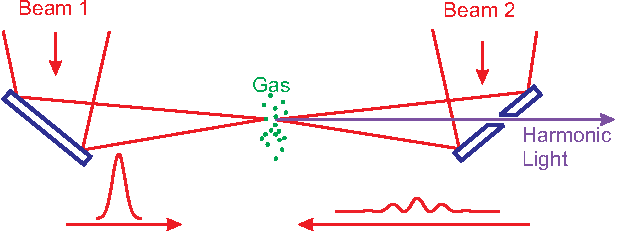
\includegraphics{Graphic1}}
    \caption[Setup for using counter-propagating light]{\label{fig:MirrorDiagram} A mirror with a hole is used to extract high-order harmonics generated in
    counter-propagating laser beams.}
\end{figure}

\begin{figure}
\centerline{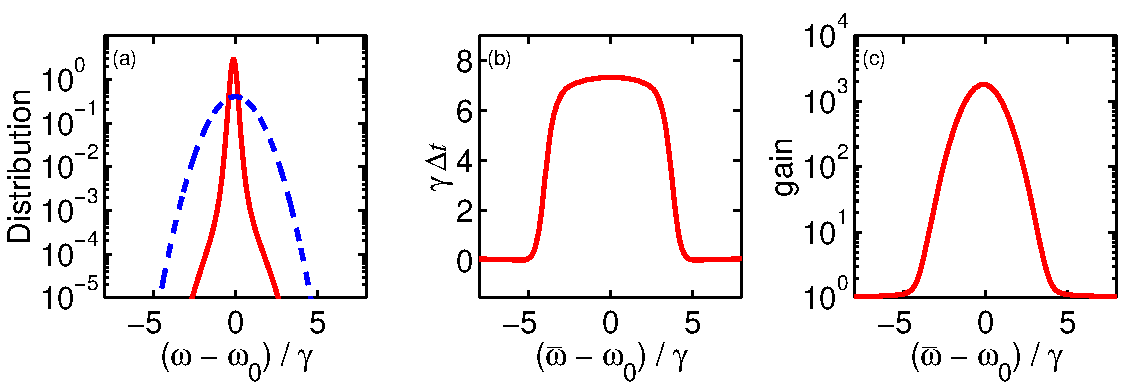
\includegraphics[width=5.5in]{Figure3}} \caption[Group
delay for broadband pulses]{\label{fig:DelayPlot} (a) Normalized
spectral distribution $\rho$ for the broadband pulse centered on
resonance before (dotted) and after(solid) propagation. (b) Total
delay as a function of $\bar{\omega}$ for the broadband pulse. (c)
Overall pulse transmission as a function of $\bar{\omega}$}
\end{figure}

 \chapter{Clear Thinking}
\label{chap:ClearThinking}

\section{Creating an outline}
\label{sec:Outline} \index{Outline}

Once you identify your research project, you should immediately
begin the writing process. The initial writing process may begin in
your lab notebook. (A good physicist keeps a lab notebook or
journal.) Make an outline (as best you can envision) of your thesis.
An example of such an outline is shown in Table~\ref{table:outline}.
In this example, the primary student research project is represented
in section~2.3. The student will work on a spectrometer which is
just one part of a larger research project involving other group
members. Nevertheless, the thesis will encompass the overall purpose
and results of the entire project (even though this will overlap
with theses written by other students). Other students, for example,
may have developed the equipment described in sections~2.1 or 2.2,
and so these items would naturally be emphasized in detail by them
(in their theses).

\begin{table}
 \renewcommand{\baselinestretch}{1}\scriptsize
\textbf{Title:} Development of a Spectrometer to Study the Influence
of Counter-Propagating Light on High-Order Harmonic Generation

\scriptsize
\begin{tabular}{p{1.8in}p{1.8in}p{1.8in}}

  %\hline
  \\
  \textbf{Chapter 1:} Introduction  & \textbf{Chapter 2:} Experimental Setup & \textbf{Chapter 3:} Results \\
  & & \\
  \raggedright

  1.1 Overview

  1.2 Background

  1.2.1 Laser Harmonic Generation

  1.2.2 High Harmonic Generation

  1.2.3 Phase Matching and Conversion Efficiency

  1.3 Using Counter-Propagating Light to Manipulate Phase Matching

  &

  \raggedright

  2.1 Laser System and Pulse Characteristics

  2.2 Experimental Setup

  2.3 High Harmonics Spectrometer

  2.3.1 Design Overview

  2.3.2 Diffraction Grating

  2.3.3 Imaging Issues

  2.3.4 Positioning Controls

  2.4 Detection

  &

  \begin{raggedright}

  3.1 Measurement of High Harmonics

  3.2 Influence of Counter-Propagating Light

  3.3 Interpretation of Results

  3.4 Conclusion and Future Outlook

  \end{raggedright}

  \\ & & \\
\end{tabular}
\renewcommand{\baselinestretch}{1.66}\small\normalsize
\caption{\label{table:outline} Sample outline for a senior thesis.}
\end{table}

The overview section (1.1) should motivate the reason for the
research without relying on specific background that will be
introduced in the later sections. You should include general
motivational statements (that you might give, for example, to a
science news reporter) as in the following example: ``Laser
high-order harmonic generation is a unique source of directional and
bright extreme ultraviolet radiation (EUV). This short wavelength
light source may have future applications in ultrafine resolution
photolithography. Because the high harmonics are coherent and
generated with short pulse lasers, they can be used to probe
ultrafast phenomena when high-energy photons are needed..." The
overview should also provide the reader with a clear demarcation of
the scope of your contribution to the overall project.

Near the end of Chapter~1, as you narrow to the specific problem to
be addressed, be sure to provide a more detailed outline of the
overall project than was given in the opening section. Again, be
specific about your role in the project. Briefly introduce and
summarize what will be discussed in the remainder of the thesis. As
is evident, the content of the first chapter depends strongly on
what is written in subsequent chapters. Therefore, the first chapter
is typically the last chapter to be completed. Nevertheless, it
should also be one of the first chapters that you begin to write.

It may happen that, while a student makes a meaningful contribution
to the overall project, the final results are not obtained before
the senior thesis is submitted. This is not ideal, but this happens
to students quite often. In this situation, the final chapter might
be entitled ``Discussion." If attempts were made at obtaining data,
the concluding chapter might describe the reasons (especially
reasons involving physics) why the attempts were unsuccessful. The
final chapter should provide suggestions on how to remedy the
situation (which can be helpful to future students who continue the
project). If the data-taking stage is not reached, the concluding
chapter might describe preliminary checks of equipment and expected
roles for the new equipment in the overall project.

The format suggested in Table~\ref{table:outline} is very flexible
and would likely be somewhat different, for example, in the case of
a thesis based on theoretical work. You should decide what works
best for you in consultation with your advisor. You may want to
examine several senior theses written by previous students which are
available in the physics department reading room (N288). There are
examples of good and not-so-good theses there. Exemplary theses were
written by Shannon Lunt, Deborah Paulsen, and Michael Ware.

\section{Importance of feedback}
\label{sec:Feedback}

Obtain feedback at every step of the writing process. Go over your
outline with your advisor. It is much less painful to rearrange or
to delete sections before you write them, when they are represented
merely in outline form. Make brief notes indicating what will go
into each section (e.g. a summary of research by Group X and Y, a
schematic of an experimental setup, a blowup view of a critical
part, etc.). Discuss your initial ideas and brainstorm together with
your advisor.

You should start writing portions of your thesis early, even though
some sections will need to wait until after the research is
concluded. When possible, begin making figures---even hand-drawn
sketches in your lab notebook. Remember to develop the overall
outline before writing specific sections. This helps to avoid
writing material that might later have to be discarded. As you write
portions of your thesis, show them to your advisor and to other
members in your research group for valuable feedback. Your advisor
will be much happier reviewing short pieces of your writing
periodically, as opposed to reviewing it all at once near the due
date. As you receive feedback along the way, you can apply it to
sections not yet written. The periodic feedback helps you to revise
and reshape your outline continually and guides you in developing a
clear scientific writing style. The writing process forces you to
organize your thoughts and to keep a clear vision of your research.
This helps you to avoid long periods of stagnation by bringing to
the foreground the next logical step in the research. The important
thing is to keep moving forward. No matter what, you will make many
mistakes, so try to make them as fast as you can. This is the
difference between experience and inexperience.

\section{Audience}
\label{sec:Audience}

You should consider as your audience the other students in your
research group. In particular, after you graduate, your thesis might
be used as a resource for students who will move into your former
role. Avoid making your thesis too basic; you may assume a certain
level of sophistication on the part of the reader. However, the
thesis should be easily understandable to a physics professor whose
research expertise is in a different field.

\section{Coherence}
\label{sec:Coherence}

Just as the overall outline of the thesis should have a clear and
logical organization, the sequence of information presented in each
section and paragraph should also follow a logical flow. Continually
ask yourself which paragraphs should appear before others. You
should be aware of a key sentence in each paragraph which usually
appears near the beginning and defines what the paragraph is
conveying. If a paragraph is very lengthy, don't hesitate to break
it into two (at a logical place). Read your own writing for logical
progression and for smoothness. Develop the skill of crafting smooth
transitions.

\section{Conciseness}
\label{sec:Concise}

Cut out the lard. Avoid long strings of prepositional phrases in
sentences of theses written by students in their senior year for the
physics department at BYU as a graduation requirement for the degree
of Bachelor of Science. (Did you get the joke?) Use simple
declarative sentences often, but not exclusively. Make every word
count. Vary sentence length. Intermingle short with long sentences
in an aperiodic fashion. You might inadvertently kill a reader with
boredom if your sentences all have the same length.

In your writing, be as quantitative as the subject matter permits,
and avoid inexact word usage. Continually ask yourself how your
writing might be misinterpreted. Make sure that arguments are
logically complete.

\section{Active voice}
\label{sec:ActiveVoice}

Remember that active verb construction generally captures the
reader's attention more than does passive construction. This does
not mean that passive voice should never be used. Just keep in mind
that an over reliance on passive verb construction results in a
rather bland document.

\section{Document format}
\label{sec:Format} \index{Format}

This document has been written following the format requested for
your thesis. Use a 12 point serif font such as Times for the main
text. If you desire variation, you can use a sans serif font such
as Helvetica for chapter and section headings. Set the margins to
one inch on all sides. Allow the right-hand side of the text to run
ragged if you use a regular word processor; text is easier to read
if it is not stretched and compressed in order to create a straight
right margin. LaTeX is a little fancier in its hyphenation and word
spacing and can usually pull of full justification fine. Double
space your lines. This makes the text easier to read and allows for
the insertion of mathematical expressions into the text without
disrupting the line spacing.

Use page breaks judiciously so that section headings do not become
isolated from their subsequent text on the bottom of a page.
Strategic positioning of figures within the text can help to avoid
large white spaces created when a figure's size forces it onto the
next page. If possible, you should avoid inserting figures before
they are discussed in the text. Your document should be printed
single-sided if it is less than 50 pages. However, if preferred you
may position figures on the backs of pages if this facilitates
keeping them close to the text describing them (located on the
adjacent page).

This document was prepared using LaTeX.  Many professors and
students choose to use LaTeX or variants such as REVTeX (a form used
by APS journals like Physical Review Letters). LaTeX can be
downloaded free of charge. For more information, go to the website
of the TeX Users Group (www.tug.org). Supplementary REVTeX macros
can be obtained from the website of the American Institute of
Physics (www.aip.org). You can also use Microsoft Word and MathType
(or the built in equation editor) for equations if you prefer. Check
with you advisor to find out which option will work best for you.

\section{Appropriate length}
\label{sec:Length}

How long does a senior thesis need to be? The answer is that it
should be as long as necessary to communicate your ideas succinctly.
There is no set length. The written document is not an end in
itself, but a vehicle to convey your ideas as efficiently as
possible to the reader. However, if the main body of your thesis
(excluding title pages and appendixes) is only 10 pages, you
probably have not included sufficient context and motivation for
your work. If the main body of your thesis exceeds 30 pages, you are
probably not concise enough. Professors and others don't really want
to read a lot of pages. A long thesis may also mean that you have
done more work than expected. Remember, you are not asked to
complete a masters project, rather a comparatively modest project in
your senior year. In the example in Table~\ref{table:outline}, the
introduction chapter might have 8 pages, the experimental setup
chapter might have 11 pages (emphasizing the work actually performed
by the hypothetical student in the example), and the results chapter
might have 6 pages (assuming results are obtained through a group
effort).

\section{Deadlines}
\label{sec:Deadlines} \index{Deadlines}

You must register for 2 credit hours of Physics 498R (499R if you
are in the honors program, 492R if you are in applied physics) in
any semester before graduation (usually when you are actively
involved in the research). At the end of the semester, if the thesis
is still in progress, you will receive a T grade. Then, when your
thesis is completed, your advisor will change it to a letter grade.
In order to allow for an adequate evaluation period, your thesis
should be submitted for review at least six weeks before graduation.
(Honor's theses are required ten weeks before graduation, submitted
first to the Honor's program and then indirectly to the department.)
After the thesis has been approved and signed by your advisor, take
it to the Senior Thesis Coordinator, currently Eric Hintz. If
acceptable, the Senior Thesis Coordinator will recommend your thesis
to the Department Chair for a signature. The Coordinator will then
forward the manuscript for binding and archiving in the Physics
Department library. Be sure to make an extra copy for yourself (and
one for your advisor). Typically, these additional private copies
are not bound unless you pay for it.


 \begin{appendices}

 \chapter{Things that belong in an appendix}
\label{app:BelongInApp}

The purpose of an appendix is to provide supplementary information
which would distract if included in the main body of the thesis.
Items appearing as an appendix might include lengthy derivations.
If students feel compelled to include a brief tutorial on relevant
background information (not new research), it should appear as an
appendix. An appendix might consist of portions of unique computer
code that was developed as part of the project.

 \chapter{Presenting a talk}
\label{app:Talk}

When presenting your thesis work in a talk, you will want to convey
an overview of your thesis as a whole. However, you must pick and
choose what to emphasize since time will be limited. There is no
formal oral defense requirement for the senior thesis (although
there is for an Honor's Thesis). However, the department encourages
students to make at least one formal presentation on their research.
All students doing a senior thesis, and especially those receiving
department funding, are expected to participate in the annual Spring
Research Conference held each March in the College of Physical and
Mathematical Sciences at BYU. Depending on available travel
resources, students may also have the opportunity to present a talk
at a professional meeting outside of campus.

For short talks, you should have no more than two thirds as many
slides as you have minutes allocated for your talk. For longer
talks, you should have somewhat fewer slides. Create a title page
which acknowledges everyone who has contributed to the work. Prepare
an outline slide that will let the audience know what you are going
to be presenting. (If time is extremely short (e.g. 7 minute talk),
you may dispense with the outline slide.) At least a third of your
talk should be introductory in nature, providing background that
will help the audience appreciate the work. The main goal in giving
a talk is to convey to the audience a sense that your work is
important; the goal is not to give the audience a lot of details
which they will never remember nor even get straight in the first
place. Less is more. A conclusion slide can be used to remind the
audience of your main points and to summarize the significance of
your work. Keep it brief. The conclusion slide may be omitted if it
seems too redundant, depending on how you presented the
material[10].

\begin{figure}
    \centerline{\includegraphics[width=6.5in]{slide}}
    \caption{\label{fig:Slide} A sample slide from a presentation}
\end{figure}

Many of the figures that you prepare for your thesis will be useful
for your slide presentation. Keep slides simple and uncluttered.
Include less information on a view graph than you plan to talk
about. Be sure that important labels are present (such as the units
on graph axes). Use large fonts so that your slides are easy to
read, even for people in the back. It is a good idea to place a
single large ``header" sentence at the top of each view graph (no
more than two lines using a 24 point font). Think of the main idea
that you want an audience member to get from a slide, and use that
for the header sentence. Use color freely, but keep it tasteful.
Figure~\ref{fig:Slide} shows an example of a view graph.

Practice your talk to yourself and to others in your research group,
especially your advisor. Time your practice runs. If you do not
practice, you will most likely give too many extraneous details and
muddle through or even miss your main points for lack of time, a
sure recipe for a boring talk.


 \end{appendices}

 \bibliography{references}

 \printindex


\end{document}
